% compile using
%> pdflatex explanation.tex
%> pdflatex explanation.tex

\documentclass[12pt,a4paper]{article}

\title{Ray intersection calculations} 

\author{KVNG Vikram}
\date{}

% giving margins
\usepackage[inner=1.25in, outer=1.25in, top=1in, bottom=1.25in]{geometry}
% for justifying without hyphens
\hyphenchar\font=-1
\sloppy
% For including images
\usepackage{graphicx}
\graphicspath{ {./} }
% For subfigures
\usepackage[labelfont=bf]{caption}
\usepackage{subcaption}
% while splitting,aligning,referencing equations Source: https://tex.stackexchange.com/questions/35295/how-can-i-number-a-few-equations-together
\usepackage{amsmath}
% For bold math symbols
\usepackage{bm}
% For hyperlinks
\usepackage{hyperref}
\hypersetup{
    colorlinks=true,
    linkcolor=black,
	citecolor=blue,
    urlcolor=blue
}

\begin{document}
\maketitle

For calculating the intersection lengths of each ray with each voxel for matrix $\bm A$, all the equations of lines and equations of the 6 surfaces of all the voxels are calculated and intersection points of each line with each of these planes are found. For each line and voxel pair there exist 6 intersection points. If a line intersects a voxel then among the 6 intersection points for that line-voxel pair 2 of the points will be on the surfaces of the voxel and rest of the 4 not on the surfaces of voxels. Distance between the 2 points on the surfaces of voxel is the intersection length for the line-voxel pair. If none of the 6 points are on the surfaces of the voxel, then the line is not intersecting the voxel. The number of points on the surfaces of voxel can either be 2 or 0 and it is never possible for any point to be inside the voxel. If the receiver for a line is inside the voxel then the line will be intersecting the voxel and among the 2 points on the voxel, only the one towards the satellite should be considered and the length of the intersection is distance between receiver to that point.  \\

If a voxel extends from limits $x_1-x_2$, $y_1-y_2$ and $z_1-z_2$ in x, y and z directions, then to check weather a point at $(x_p,y_p,z_p)$ is present on the surface three conditions can be used. They are
\begin{equation} \label{eq:ideal_intersection_conditions}
	\begin{aligned}
	x_1 <= x_p <= x_2 \\
	y_1 <= y_p <= y_2 \\
	z_1 <= z_p <= z_2
	\end{aligned}
\end{equation}
If all three of these conditions are satisfied then the point is on the surface of the voxel. \\

\begin{figure}[p]
	\centering

	\begin{subfigure}[t]{0.45\textwidth}
		\centering
		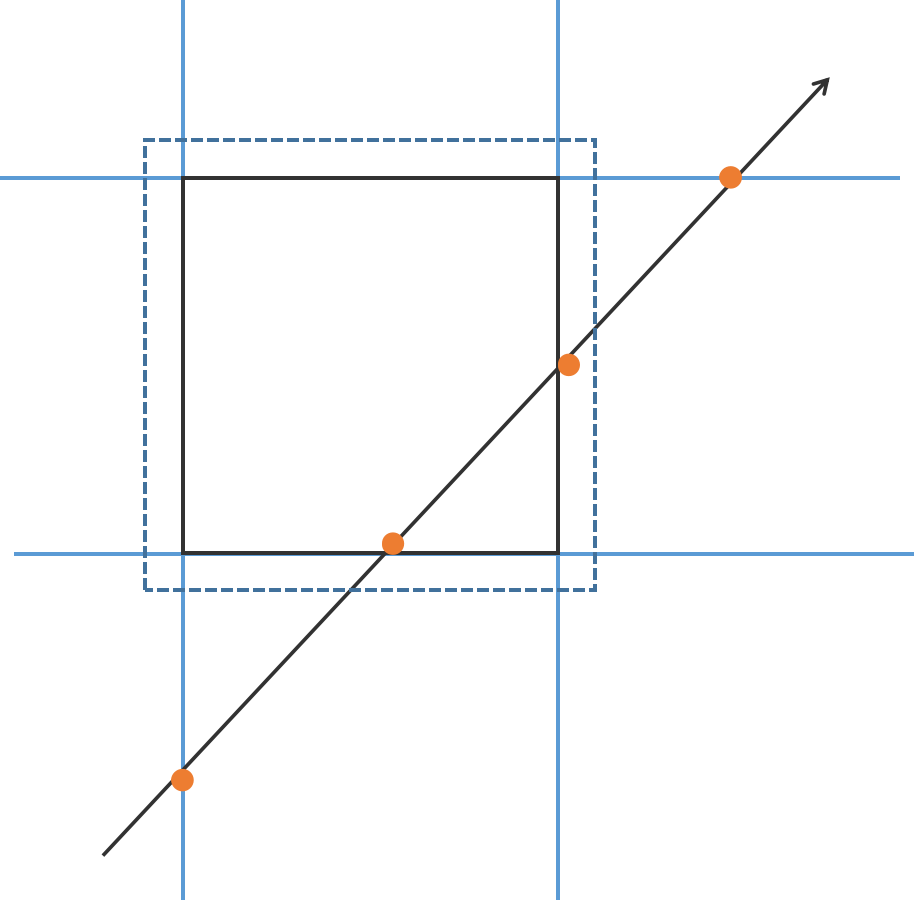
\includegraphics[width=0.8\linewidth]{ray_ordinary}
		\caption{No adjustments needed.}
		\label{fig:ray_ordinary}
	\end{subfigure}
	\hfill
	\begin{subfigure}[t]{0.45\textwidth}
		\centering
		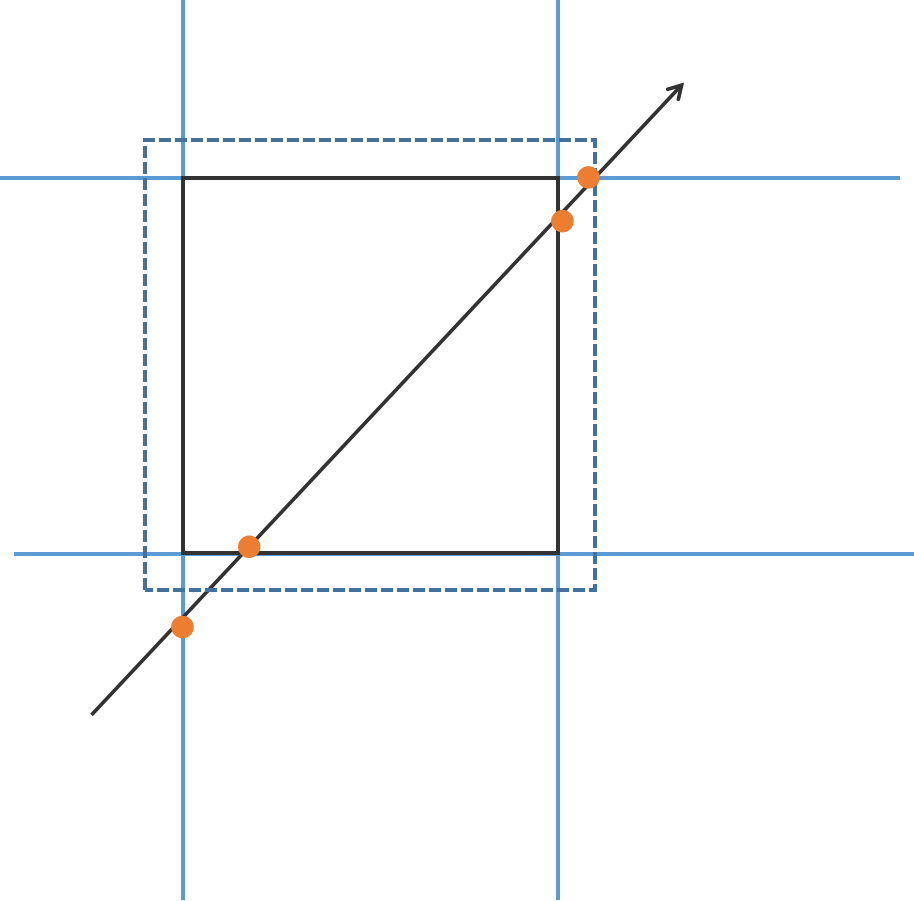
\includegraphics[width=0.8\linewidth]{ray_working}
		\caption{Adjustments happen until only 2 points are included.}
		\label{fig:ray_working}
	\end{subfigure}
	\medskip % to give a space between sub figure rows

	\begin{subfigure}[t]{0.45\textwidth}
		\centering
		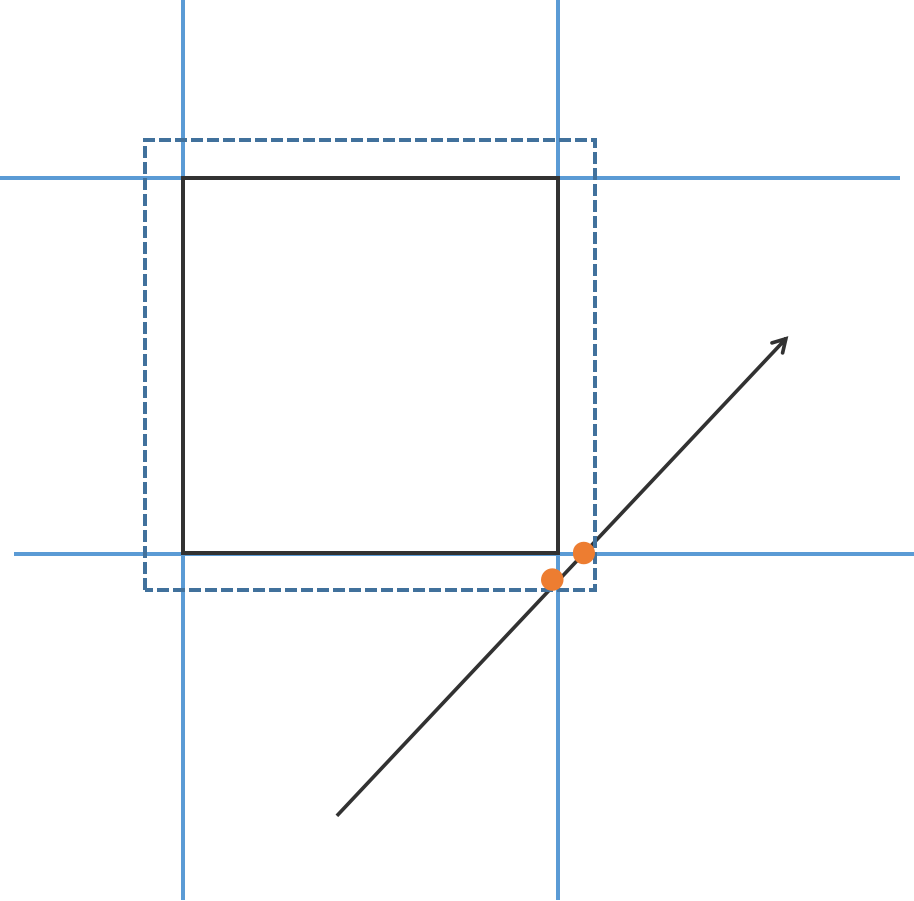
\includegraphics[width=0.8\linewidth]{ray_negligible_1}
		\caption{If 1 point is included then adjustment happens until 2 are included, leading to a minute error.}
		\label{fig:ray_negligible_1}
	\end{subfigure}
	\hfill
	\begin{subfigure}[t]{0.45\textwidth}
		\centering
		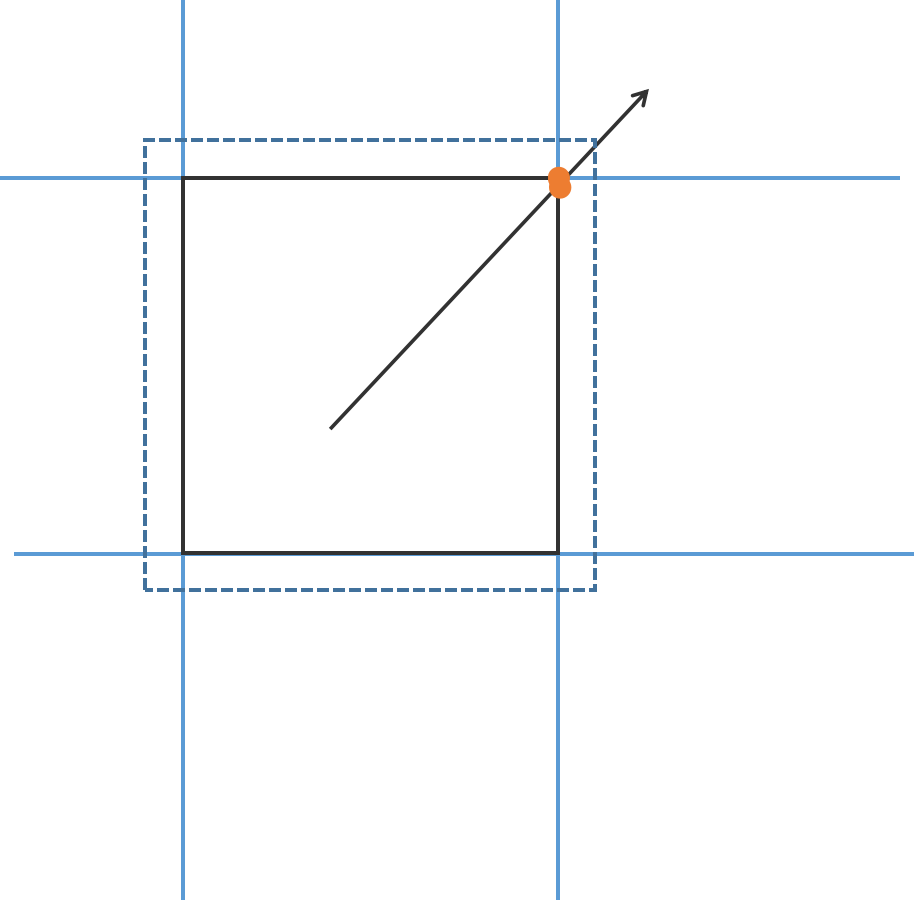
\includegraphics[width=0.8\linewidth]{ray_negligible_2}
		\caption{With receiver inside voxel, adjustment happens until only 1 point is included.}
		\label{fig:ray_negligible_2}
	\end{subfigure}
	\medskip % to give a space between sub figure rows

	\begin{subfigure}[t]{0.45\textwidth}
		\centering
		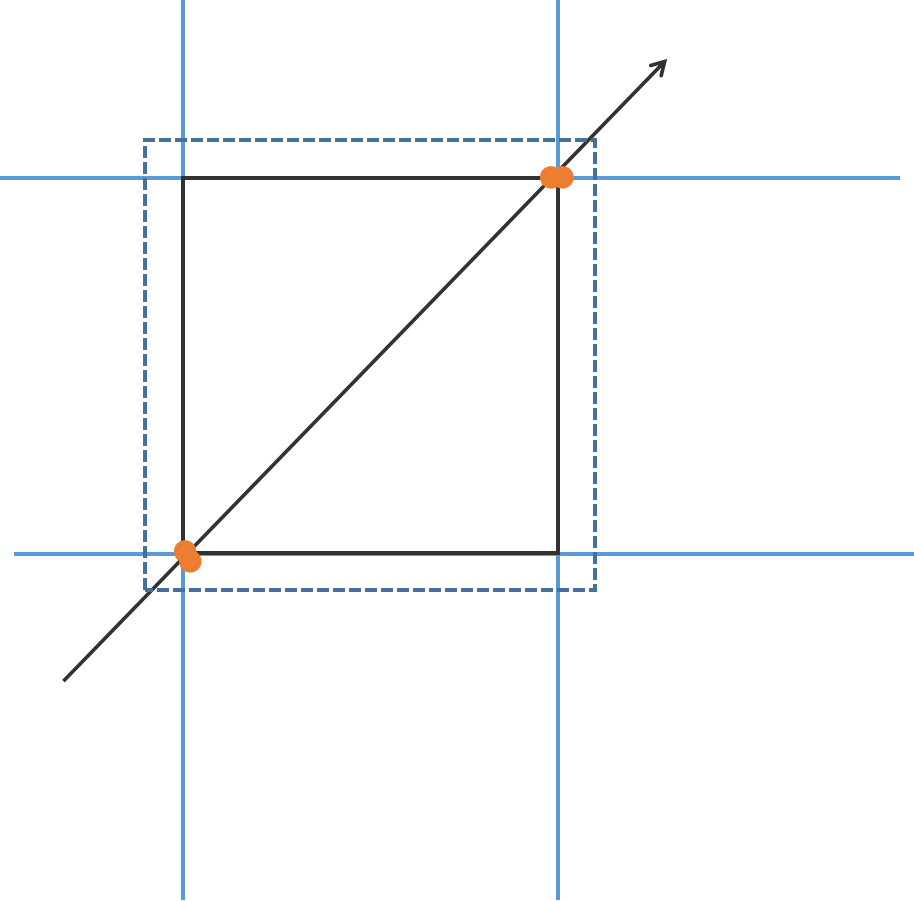
\includegraphics[width=0.8\linewidth]{ray_edge_case_1}
		\caption{In very rare cases, when precision errors are greater than distances between points, adjustments may not work.}
		\label{fig:ray_edge_case_1}
	\end{subfigure}
	\hfill
	\begin{subfigure}[t]{0.45\textwidth}
		\centering
		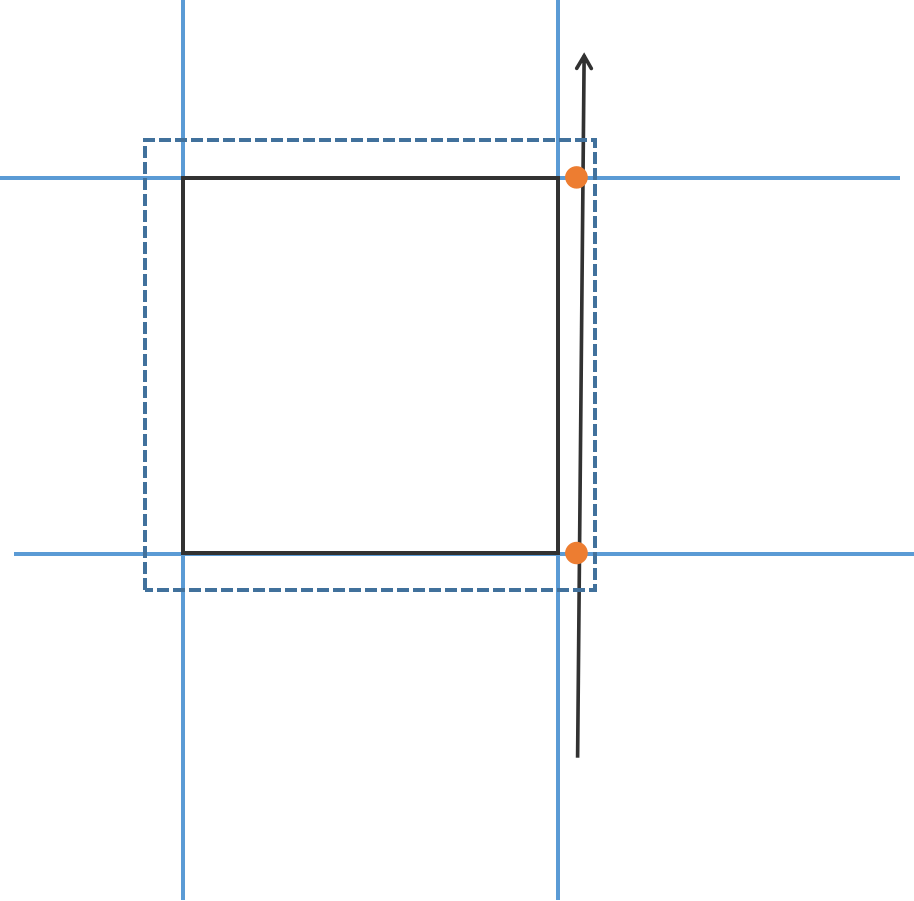
\includegraphics[width=0.8\linewidth]{ray_edge_case_2}
		\caption{Edge case with false positive intersection.}
		\label{fig:ray_edge_case_2}
	\end{subfigure}
	\medskip % to give a space between sub figure rows

	\caption{Example scenarios of line-voxel intersections in 2D. Blue lines are planes forming voxels, dotted lines are the region included with margins, black arrow is ray and orange dots are intersection points.}
	\label{fig:ray_intersections}

\end{figure}

Even the calculations for line and plane intersections are simple, it may be possible that due to precision errors the intersection point may not be exactly on the surface of voxel. Even though these precision errors are negligible for intersection length calculations, there can be problems while applying the conditions mentioned above. For the conditions to work on these cases they are modified by including a margin $m$ such that the new conditions are
\begin{equation}
	\begin{aligned}
	x_1-m <= x_p <= x_2+m \\
	y_1-m <= y_p <= y_2+m \\
	z_1-m <= z_p <= z_2+m
	\end{aligned}
\end{equation} \\	

A constant value for $m$ may not work in all the cases leading to not selecting exactly 2 points or exactly 0 (or 1 if receiver is inside the voxel) from the 6 intersection points. So the margin is iteratively adjusted to get the correct number of intersection points. When the number of points included in the selection region is less than what they are supposed to be, $m$ is incremented and if more points are included then $m$ is decreased. These adjustments happen with an initial step value and when it is overdone, the step value is reduced by a factor and adjustments happen in reverse direction. When the receiver is inside the voxel then there should be only one intersection point, and if they are any number more or less than adjustments are made to make it 1. For cases where receiver is not inside the voxel, if the number of points included is 1 then adjustments are made until it becomes 2, if number of points included is more than 2 then adjustments are made until they become 2 and if number of points included is 0 then no adjustments are make. \\

Fig. \ref{fig:ray_intersections} shows different scenarios faced by the adjustment mechanism. In most cases adjustments happen without any mistakes since a plane line intersection is mathematically simpler. If the voxels are not taken as perfect cuboids but as made of non-plane surfaces like constant latitude, longitude and height surfaces then precision errors become a more serious problem and adjustments may still do mistakes but that is not the case here. Among all the cases shown is Fig. \ref{fig:ray_intersections}, Fig. \ref{fig:ray_edge_case_1} and Fig. \ref{fig:ray_edge_case_2} are the edge cases with large errors but these are very rare (never occurred yet). The initial value of margin $m$ is taken as 0.01 m which is very small compared to km scale voxels, so any other small errors are not a problem for km scale distances. \\

After the ray intersection length calculations are done they can be easily verified for errors by checking if the sum of individual intersection length of a ray is equal to the distance between the starting point and ending point in the grid. If there are any mistakes then those rays can be excluded or corrected. \\

\end{document}
